% PREAMBLE
\documentclass{ieeeaccess}
\usepackage{cite}
\usepackage{amsmath,amssymb,amsfonts}
\usepackage{algorithmic}
\usepackage{graphicx}
\usepackage{textcomp}
\usepackage{booktabs}
% ieeeaccess.cls redefines \year, which pgf needs as the TeX primitive
\let\accessyear\year
\protected\def\year{\pdfprimitive\year}
\usepackage{tikz}
\usetikzlibrary{positioning,arrows.meta,calc}
\let\year\accessyear
% captions of plain figure environments read \xfigwd, set by the class's \Figure
\def\xfigwd{0pt}
% xcolor (loaded by TikZ) cannot use the class's Pantone spot color, so use its CMYK equivalent
\definecolor{accessblue}{cmyk}{1,0.3,0,0.2}
\def\BibTeX{{\rm B\kern-.05em{\sc i\kern-.025em b}\kern-.08em T\kern-.1667em\lower.7ex\hbox{E}\kern-.125emX}}
\newcommand{\todo}[1]{\textcolor{red}{[TODO: #1]}}
% DOCUMENT
\begin{document}
% FRONT MATTER: TITLE, AUTHORS, AFFILIATIONS
\history{Date of publication xxxx 00, 0000, date of current version xxxx 00, 0000.}
\doi{10.1109/ACCESS.2017.DOI}

\title{StorageLab: A Verifiable, Hardware-Independent Laboratory for RAID, Disk Performance, and Data Protection Education}
\author{\uppercase{First Author}\authorrefmark{1}, \uppercase{Second Author}\authorrefmark{1}, \uppercase{and Third Author}\authorrefmark{1}}
\address[1]{\todo{Department, Institution, City, Country} (e-mail: \todo{e-mail})}
\tfootnote{\todo{Funding or support statement, if any.}}

\markboth {Author \headeretal: StorageLab: A Verifiable Laboratory for Storage Systems Education} {Author \headeretal: StorageLab: A Verifiable Laboratory for Storage Systems Education}

\corresp{Corresponding author: \todo{Name} (e-mail: \todo{e-mail}).}

% ABSTRACT
\begin{abstract}
Core storage concepts such as parity, degraded operation, rebuild, queueing delay, recovery objectives, and replication lag are usually taught with static diagrams, because enterprise arrays and multi-site links are not available in a classroom. Production tools hide the block layout and require privileged access, while online calculators return numbers without a derivation or any failure behavior. This paper presents StorageLab, a hardware-independent, web-based laboratory that combines five analytical models with a block-level redundant array of independent disks (RAID) engine. The models cover RAID capacity and failure states, single-disk queueing performance, backup storage with recovery point and recovery time compliance, synchronous and asynchronous replication, and likelihood-impact risk. The engine stripes a real user file across one file per simulated disk using RAID 0, 1, 5, 6, or 10. RAID 5 uses rotating exclusive-or parity, and RAID 6 adds a Reed-Solomon syndrome over the Galois field of 256 elements. A disk failure is injected by deleting its file. The engine then reads in degraded mode, rebuilds onto a hot spare with streamed progress, and proves recovery by comparing the SHA-256 digest of the reassembled file with the original. Every analytical result carries its units, stated assumptions, and a rule-based explanation generated from the same formulas. An exhaustive fault-injection campaign over 1,058 failure combinations across 14 array configurations found zero silent corruptions, and the engine's recoverability predicate agreed with the observed outcome in every case. For a 4 MiB file, every engine operation completes within 25 ms on a laptop, without special privileges.
\end{abstract}

% INDEX TERMS
\begin{keywords}
Backup and recovery, computer science education, erasure coding, Galois fields, queueing theory, RAID, Reed-Solomon codes, replication, simulation, storage systems.
\end{keywords}

\titlepgskip=-15pt

\maketitle

% I. INTRODUCTION
\section{Introduction}
\label{sec:intro}
\PARstart{S}{torage} management courses ask students to reason about mechanisms they almost never see operate. Parity reconstruction, degraded reads, rebuild onto a hot spare, the queueing delay that grows as a disk approaches saturation, the recovery point objective (RPO) and recovery time objective (RTO) of a backup plan, and the lag of asynchronous replication are normally presented as static diagrams in textbooks such as \cite{emc2012ism}. The equipment that exhibits these behaviors, such as enterprise disk arrays, storage area network fabrics, and multi-site links, is expensive and rarely available in a teaching laboratory.

The software that does exist is not built for teaching. Production RAID implementations, such as the Linux multiple-device driver or hardware controllers, are correct and fast but opaque: they hide the block layout, require root access or real block devices, and give no account of why an array reached a particular state. Research simulators such as DiskSim \cite{bucy2008disksim} model devices accurately but target researchers and provide no learner-facing explanation. Online capacity and IOPS calculators return a single number, with no derivation and no way to observe failure.

As a result, no single, lightweight tool lets a learner both (a) compute textbook storage metrics with visible formulas and (b) watch the same concepts execute on real bytes, with a checkable proof of correctness, on an ordinary laptop and without special privileges. This paper addresses that gap with StorageLab and asks three research questions:
\begin{itemize}
\item RQ1: Can a pure-software, file-backed RAID engine demonstrate RAID 0, 1, 5, 6, and 10 failure and recovery faithfully enough to be verifiable, meaning byte-exact recovery within the fault tolerance and correctly reported data loss beyond it?
\item RQ2: Can analytical storage models be presented so that every output is traceable to a formula, its units, and its assumptions?
\item RQ3: Is the system light enough to run interactively on commodity hardware?
\end{itemize}

The contributions of this work are as follows.
\begin{enumerate}
\item A block-level, file-backed RAID engine implementing RAID 0, 1, 5 (rotating XOR parity), 6 (P parity plus a Reed-Solomon Q syndrome over GF($2^8$) with reduction polynomial 0x11D and generator 2), and 10. It supports degraded reads, hot-spare rebuild streamed as newline-delimited JSON (NDJSON), and SHA-256 end-to-end verification.
\item A closed-form treatment of every RAID 6 two-erasure case (data and data, data and P, data and Q, P and Q), each checked by exhaustive fault injection.
\item An integrated set of textbook storage models (an M/M/1 disk, backup storage and RPO/RTO compliance, replication latency and lag, and likelihood-impact risk), each exposed as a REST endpoint that returns values, units, assumptions, and a deterministic, formula-grounded explanation.
\item A layered architecture in which the same calculation functions drive two front ends and a test suite.
\item A validation methodology based on exhaustive enumeration of failure subsets, a recoverability predicate checked against observed behavior, and hand-calculated formula tests, which produced 1,058 of 1,058 agreements and zero silent mismatches.
\end{enumerate}

The rest of the paper is organized as follows. Section~\ref{sec:related} reviews related work. Section~\ref{sec:arch} describes the system architecture. Section~\ref{sec:engine} presents the RAID engine and its correctness argument. Section~\ref{sec:models} describes the analytical models and the explanation layer. Section~\ref{sec:eval} reports the validation and results. Section~\ref{sec:disc} discusses limitations, and Section~\ref{sec:concl} concludes.

% II. RELATED WORK
\section{Related Work}
\label{sec:related}

% II-A. RAID and Erasure Coding
\subsection{RAID and Erasure Coding}
Patterson, Gibson, and Katz introduced redundant arrays of inexpensive disks and the numbered RAID levels \cite{patterson1988raid}. Chen \emph{et al.} later surveyed RAID performance and reliability in depth \cite{chen1994raid}. RAID 6 extends single parity to tolerate two concurrent failures. Its common construction uses the Reed-Solomon codes of \cite{reed1960polynomial}, whose application to RAID-like systems was made accessible by Plank's tutorial \cite{plank1997tutorial}. The Linux kernel's RAID 6 implementation, described by Anvin \cite{anvin2004raid6}, fixes the field GF($2^8$) with the reduction polynomial $x^8+x^4+x^3+x^2+1$ and the generator $g=2$. StorageLab adopts the same convention, so a student who studies its engine also learns the arithmetic used in a widely deployed production system.

% II-B. Disk and Queueing Models
\subsection{Disk and Queueing Models}
Ruemmler and Wilkes describe the components of disk service time, namely seek, rotational latency, and transfer, and the trade-offs between simple and detailed disk models \cite{ruemmler1994disk}. Classical queueing theory \cite{kleinrock1975queueing} and Little's law \cite{little1961proof} relate utilization, response time, and the number of requests in the system. StorageLab uses the single-server M/M/1 form of these results because it is the form taught in introductory storage courses \cite{emc2012ism}. DiskSim \cite{bucy2008disksim} provides far higher fidelity but is aimed at researchers and requires detailed device parameters.

% II-C. Tools for Systems and Storage Education
\subsection{Tools for Systems and Storage Education}
\todo{Survey simulation and visualization tools used in operating systems, storage, and networking education. Cite only works that have been located and read.}

% II-D. Positioning
\subsection{Positioning}
DiskSim-class simulators are accurate but research-oriented and offer no learner-facing explanations. Linux md and hardware RAID are real but opaque and need privileges. Online calculators provide numbers without failure behavior or proof. StorageLab combines executable RAID on real bytes, hash-verified recovery, formula-traceable models, and explanations in a single tool that runs on a laptop.

% III. SYSTEM ARCHITECTURE
\section{System Architecture}
\label{sec:arch}

% III-A. Layers
\subsection{Layers}
StorageLab follows a three-layer design, shown in Fig.~\ref{fig:arch}. A React 19 and TypeScript single-page application communicates over JSON REST, plus an NDJSON stream for rebuild progress, with a FastAPI back end. The routers validate requests, call the calculation modules, and annotate the results. Every formula lives in the calculation modules. Saved experiments are stored in SQLite, and each live RAID array is stored as a directory of disk files.

\begin{figure}[!t]
\centering
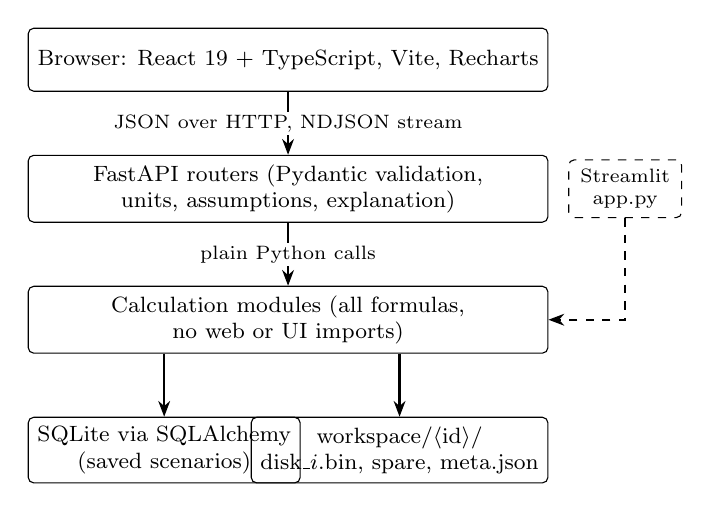
\begin{tikzpicture}[box/.style={draw, rounded corners=2pt, align=center, font=\footnotesize, minimum width=6.6cm, minimum height=0.8cm}, sbox/.style={draw, rounded corners=2pt, align=center, font=\footnotesize, minimum width=3.1cm, minimum height=0.8cm}, arr/.style={-{Stealth[length=2mm]}, thick}, lab/.style={font=\scriptsize, fill=white, inner sep=1pt}]
\node[box] (ui) {Browser: React 19 + TypeScript, Vite, Recharts};
\node[box, below=0.8cm of ui] (api) {FastAPI routers (Pydantic validation,\\ units, assumptions, explanation)};
\node[box, below=0.8cm of api] (mod) {Calculation modules (all formulas,\\ no web or UI imports)};
\node[sbox, below=0.8cm of mod.south west, anchor=north west] (db) {SQLite via SQLAlchemy\\ (saved scenarios)};
\node[sbox, below=0.8cm of mod.south east, anchor=north east] (ws) {workspace/$\langle$id$\rangle$/\\ disk\_$i$.bin, spare, meta.json};
\draw[arr] (ui) -- node[lab] {JSON over HTTP, NDJSON stream} (api);
\draw[arr] (api) -- node[lab] {plain Python calls} (mod);
\draw[arr] (mod.south -| db.north) -- (db.north);
\draw[arr] (mod.south -| ws.north) -- (ws.north);
\node[draw, dashed, rounded corners=2pt, font=\scriptsize, align=center, right=0.25cm of api, anchor=west, text width=1.2cm] (st) {Streamlit\\ app.py};
\draw[arr, dashed] (st.south) |- (mod.east);
\end{tikzpicture}
\caption{StorageLab architecture. The same calculation modules serve the REST API, the alternate Streamlit front end, and the test suite.}
\label{fig:arch}
\end{figure}

The code enforces three design rules. First, routers only validate, call, and annotate; React pages contain no formulas. Second, each module's Streamlit renderer imports Streamlit inside the function, so the calculation functions can be imported and tested without any user interface dependency. Third, validation runs twice: Pydantic bounds at the API edge and semantic checks in the module, such as minimum disk counts, even counts, and utilization below one. A module \texttt{ValueError} is mapped to HTTP 422 by a global exception handler.

% III-B. Technology Stack
\subsection{Technology Stack}
Table~\ref{tab:stack} lists the technology stack and the versions measured on the evaluation machine. The tracked code consists of 2,677 lines of Python, 2,242 lines of TypeScript and TSX, and 1,887 lines of CSS.

\begin{table}[!t]
\caption{Technology Stack}
\label{tab:stack}
\centering
\footnotesize
\setlength{\tabcolsep}{4pt}
\begin{tabular}{p{2.0cm}p{5.8cm}}
\toprule
Layer & Technology \\
\midrule
Back end & Python 3.15.2, NumPy 2.5.5, pandas 3.1.1 \\
API & FastAPI 0.165.0, Pydantic 2.14.4, Uvicorn \\
Persistence & SQLAlchemy 2.1.9, SQLite (PostgreSQL configurable) \\
Front end & React 19.3, TypeScript 7.0, Vite 8.3, Recharts 3.11, React Router 7, TanStack Query 5 \\
Alternate UI & Streamlit 1.67.0, Plotly \\
Testing & pytest, httpx, Vitest 5, Testing Library, jsdom \\
Deployment & Docker (Python API image, nginx front-end image), docker-compose \\
\bottomrule
\end{tabular}
\end{table}

% III-C. REST Interface
\subsection{REST Interface}
The API exposes one group of endpoints per module. The RAID group provides capacity calculation, failure-state simulation, an interactive XOR recovery exercise, and the live-array operations: create an array from an uploaded file, inspect its layout, fail a disk, verify, rebuild onto a spare, and delete. The disk, backup, replication, and risk groups each provide one analysis endpoint, and a scenarios group provides create, read, update, delete, clone, compare, and CSV export of saved experiments. Every analytical response has the same shape: the computed values, a \texttt{units} map, an \texttt{assumptions} list, and an \texttt{explanation} object with a summary, the formula, the contributing factors, and the assumptions.

% III-D. Front End
\subsection{Front End}
The interface has one page per module, a saved-experiments page, and a methodology page. Charts include a RAID efficiency bar chart and a disk response-time curve with a reference line at the 70\% utilization knee and a marker at the current operating point. Each module has a collapsible quick-start guide and an explanation panel, and the layout is usable at a phone width of 390 px without horizontal scrolling. The live-array panel reads the rebuild response with a stream reader, splits the NDJSON lines, and updates a progress bar; the final line carries the new array layout.

% IV. BLOCK-LEVEL RAID ENGINE
\section{Block-Level RAID Engine}
\label{sec:engine}

The RAID engine is the core technical contribution. It is about 440 lines of Python and NumPy.

% IV-A. Configuration Space
\subsection{Configuration Space}
The supported configurations are listed in Table~\ref{tab:config}. The limits keep every operation interactive and every exhaustive test tractable.

\begin{table}[!t]
\caption{Engine Configuration Space}
\label{tab:config}
\centering
\footnotesize
\begin{tabular}{p{2.0cm}p{5.6cm}}
\toprule
Parameter & Allowed values \\
\midrule
Levels & RAID 0, 1, 5, 6, 10 \\
Disks $n$ & RAID 0: $n \ge 2$; RAID 1: $n=2$; RAID 5: $n \ge 3$; RAID 6: $n \ge 4$; RAID 10: $n \ge 4$ and even; all $n \le 8$ \\
Stripe unit $b$ & 512, 1024, 4096, 16384, 65536 bytes \\
Hot spares & 0 to 2 \\
File size & 1 byte to 5 MiB \\
\bottomrule
\end{tabular}
\end{table}

% IV-B. On-Disk Representation
\subsection{On-Disk Representation}
Each array receives a 12-hexadecimal-character identifier and a directory. The file \texttt{disk\_$i$.bin} holds the concatenation of disk $i$'s blocks, row by row, and each spare is pre-allocated as zero bytes of the same size. A metadata file records the level, $n$, $b$, the number of rows, the original size and SHA-256 digest, the spares, and an event log.

Failure state is not stored. It is derived: a disk has failed if and only if its file does not exist. The physical state of the directory is therefore the single source of truth, and fault injection is simply file deletion. Identifiers must fully match \texttt{[0-9a-f]\{12\}} and the directory must contain the metadata file; any other request returns HTTP 404, which prevents path traversal.

% IV-C. Striping and Layout
\subsection{Striping and Layout}
Let $k$ be the number of data blocks per row: $k=n$ for RAID 0, $k=1$ for RAID 1, $k=n-1$ for RAID 5, $k=n-2$ for RAID 6, and $k=n/2$ for RAID 10. A file of $s$ bytes occupies \begin{equation} \text{rows} = \left\lceil \frac{s}{k\,b} \right\rceil \label{eq:rows} \end{equation} rows. The file is zero-padded to $\text{rows}\cdot k\cdot b$ bytes, viewed as an array of $\text{rows}\cdot k$ blocks of $b$ bytes, and each row's $k$ data blocks are encoded into $n$ stored blocks.

The role of each disk in row $r$ is assigned as follows. In RAID 0, disk $d$ holds data block $d$. In RAID 1 and 10, disk $d$ holds data block $\lfloor d/2 \rfloor$, so the mirror pairs are $(0,1), (2,3), \dots$. In RAID 5, P is on disk $r \bmod n$. In RAID 6, P is on disk $r \bmod n$ and Q is on disk $(r+1) \bmod n$. In RAID 5 and 6, data indices $0,\dots,k-1$ fill the remaining disks in ascending order. Fig.~\ref{fig:layout} shows the resulting layouts. This is a simple rotating-parity layout; it is not identical to the left-symmetric layout of Linux md.

\begin{figure}[!t]
\centering
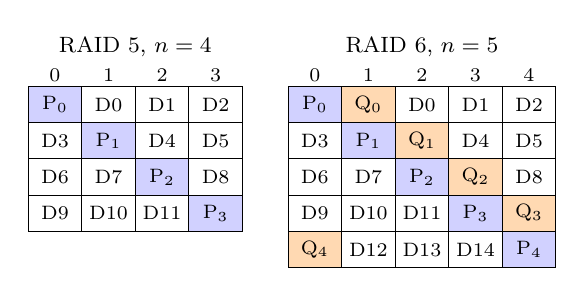
\begin{tikzpicture}[x=0.68cm, y=0.46cm, font=\scriptsize]
\tikzset{cell/.style={draw, minimum width=0.68cm, minimum height=0.46cm, inner sep=0pt}}
\tikzset{pc/.style={cell, fill=blue!18}, qc/.style={cell, fill=orange!30}, dc/.style={cell}}
% RAID 5, n = 4
\node at (1.5,1.1) {\footnotesize RAID 5, $n=4$};
\foreach \d in {0,...,3} \node at (\d,0.3) {\d};
\foreach \r/\row in {0/{pc/P$_{0}$,dc/D0,dc/D1,dc/D2}, 1/{dc/D3,pc/P$_{1}$,dc/D4,dc/D5}, 2/{dc/D6,dc/D7,pc/P$_{2}$,dc/D8}, 3/{dc/D9,dc/D10,dc/D11,pc/P$_{3}$}} {\foreach [count=\d from 0] \s/\t in \row {\node[\s] at (\d,-\r-0.5) {\t};}}
% RAID 6, n = 5
\begin{scope}[xshift=3.3cm]
\node at (2,1.1) {\footnotesize RAID 6, $n=5$};
\foreach \d in {0,...,4} \node at (\d,0.3) {\d};
\foreach \r/\row in {0/{pc/P$_{0}$,qc/Q$_{0}$,dc/D0,dc/D1,dc/D2}, 1/{dc/D3,pc/P$_{1}$,qc/Q$_{1}$,dc/D4,dc/D5}, 2/{dc/D6,dc/D7,pc/P$_{2}$,qc/Q$_{2}$,dc/D8}, 3/{dc/D9,dc/D10,dc/D11,pc/P$_{3}$,qc/Q$_{3}$}, 4/{qc/Q$_{4}$,dc/D12,dc/D13,dc/D14,pc/P$_{4}$}} {\foreach [count=\d from 0] \s/\t in \row {\node[\s] at (\d,-\r-0.5) {\t};}}
\end{scope}
\end{tikzpicture}
\caption{Rotating parity layouts used by the engine for RAID 5 with four disks and RAID 6 with five disks. Columns are disks and rows are stripes. D$i$ is the $i$-th data block of the file; P$_r$ and Q$_r$ are the parity and syndrome of row $r$.}
\label{fig:layout}
\end{figure}

% IV-D. Parity Mathematics
\subsection{Parity Mathematics}
For RAID 5 and 6 the parity block is the bytewise exclusive-or of the row's data blocks: \begin{equation} P = D_0 \oplus D_1 \oplus \dots \oplus D_{k-1}. \label{eq:p} \end{equation} RAID 6 adds the Q syndrome over GF($2^8$) with reduction polynomial $x^8+x^4+x^3+x^2+1$ (0x11D) and generator $g = 2$: \begin{equation} Q = \bigoplus_{i=0}^{k-1} g^{i} \cdot D_i , \label{eq:q} \end{equation} where multiplication is in GF($2^8$) and is applied bytewise.

Field arithmetic uses log and antilog tables built once at import time by repeated left shift with reduction by 0x11D on overflow. The antilog table has 512 entries, doubled so that the sum of two logarithms never needs a modulo. Multiplying a whole block by a constant $c$ is a single vectorized NumPy expression, $\mathrm{EXP}[\mathrm{LOG}[\text{block}] + \mathrm{LOG}[c]]$, applied to the non-zero bytes; there is no per-byte Python loop. The inverse is $g^{-1}(v) = \mathrm{EXP}[(255 - \mathrm{LOG}[v]) \bmod 255]$.

% IV-E. Row Reconstruction
\subsection{Row Reconstruction}
Reconstruction works one row at a time. Given the stored blocks of a row with some blocks missing, the engine first checks the recoverability predicate of Section~\ref{sec:pred} and raises a data-loss error if it fails. It then collects the surviving data blocks, P, and Q, and solves for the lost data indices using the cases below.

One data block $D_x$ lost and P present: \begin{equation} D_x = P \oplus \bigoplus_{i \ne x} D_i . \label{eq:rec1} \end{equation}

One data block $D_x$ lost together with P, and Q present: \begin{equation} D_x = g^{-x} \cdot \Bigl( Q \oplus \bigoplus_{i \ne x} g^{i} D_i \Bigr). \label{eq:rec2} \end{equation}

Two data blocks $D_x$ and $D_y$ lost. Define the partial parity and syndrome of the surviving data, \begin{align} P_{xy} &= P \oplus \bigoplus_{i \notin \{x,y\}} D_i = D_x \oplus D_y, \\ Q_{xy} &= Q \oplus \bigoplus_{i \notin \{x,y\}} g^{i} D_i = g^{x} D_x \oplus g^{y} D_y . \end{align} Multiplying the first equation by $g^{y}$ and adding it to the second eliminates $D_y$: \begin{equation} D_x = \frac{Q_{xy} \oplus g^{y} P_{xy}}{g^{x} \oplus g^{y}}, \qquad D_y = P_{xy} \oplus D_x . \label{eq:rec3} \end{equation}

If only P, only Q, or both are lost, no data is lost and they are recomputed from (\ref{eq:p}) and (\ref{eq:q}). For RAID 1 and 10, a lost block is copied from the surviving member of its mirror pair. After the data are recovered, the full row is re-encoded, and a rebuild takes the block that belongs to the target disk.

The denominator in (\ref{eq:rec3}) is never zero. Because $g=2$ is a primitive element of GF($2^8$), its powers $g^0,\dots,g^{254}$ are distinct. With $n \le 8$, RAID 6 has $k \le 6 < 255$ data indices, so $g^x \ne g^y$ and therefore $g^x \oplus g^y \ne 0$ for every $x \ne y$. The two-erasure system always has a unique solution.

Because parity rotates, one failed physical disk holds data in some rows and P or Q in others. The engine therefore solves each row independently. For this reason, a RAID 6 array with two failed disks exercises all four erasure cases (data and data, data and P, data and Q, P and Q) across its rows, and the exhaustive campaign in Section~\ref{sec:eval} tests all of them.

% IV-F. Recoverability Predicate
\subsection{Recoverability Predicate}
\label{sec:pred}
Let $M$ be the set of missing disks. The engine declares the array recoverable when \begin{equation} \text{rec}(M) = \begin{cases} M = \emptyset & \text{RAID 0},\\ \nexists j : \{2j, 2j+1\} \subseteq M & \text{RAID 1, 10},\\ |M| \le 1 & \text{RAID 5},\\ |M| \le 2 & \text{RAID 6}. \end{cases} \label{eq:pred} \end{equation} The array is Healthy if $M$ is empty, Degraded if $M$ is recoverable, and Failed otherwise. The guaranteed fault tolerance shown in the interface is 0, 1, 1, 2, and 1 disks for RAID 0, 1, 5, 6, and 10. RAID 10 can survive up to $n/2$ failures when each failure is in a different mirror pair.

% IV-G. Operations
\subsection{Operations}
\emph{Create} validates the configuration, pads the file, encodes all rows into an $(n, \text{rows}, b)$ array, writes each disk, allocates the spares, and records the SHA-256 digest of the original file.

\emph{Fail} deletes a disk file and appends an event to the log.

\emph{Read} checks recoverability, loads the surviving disks, recovers each row, emits the data blocks in index order, and truncates the result to the original size.

\emph{Verify} returns the state, the missing disks, the original and the read SHA-256 digests, whether they match, whether data was lost, and a message such as ``Read in degraded mode: Disk 2 reconstructed on the fly''.

\emph{Rebuild} validates eagerly (the disk must be missing, the missing set recoverable, and a spare available) and then returns a generator. The generator writes the recovered row blocks into the spare file and reports progress after each row. Only when the last row is written is the spare renamed to \texttt{disk\_$i$.bin}. An interrupted rebuild therefore never presents a half-written disk as healthy. The API throttles progress to about 50 updates and spreads an artificial delay of 2.5 s across the rows so that the progress bar is visible; the engine timings in Section~\ref{sec:eval} exclude this delay.

\emph{Layout} returns the role, label (D, D$'$, P, or Q), and the first four bytes in hexadecimal of every block for up to 12 rows, so the interface displays real stored bytes rather than a mock-up (Fig.~\ref{fig:live}).

\begin{figure}[!t]
\centering
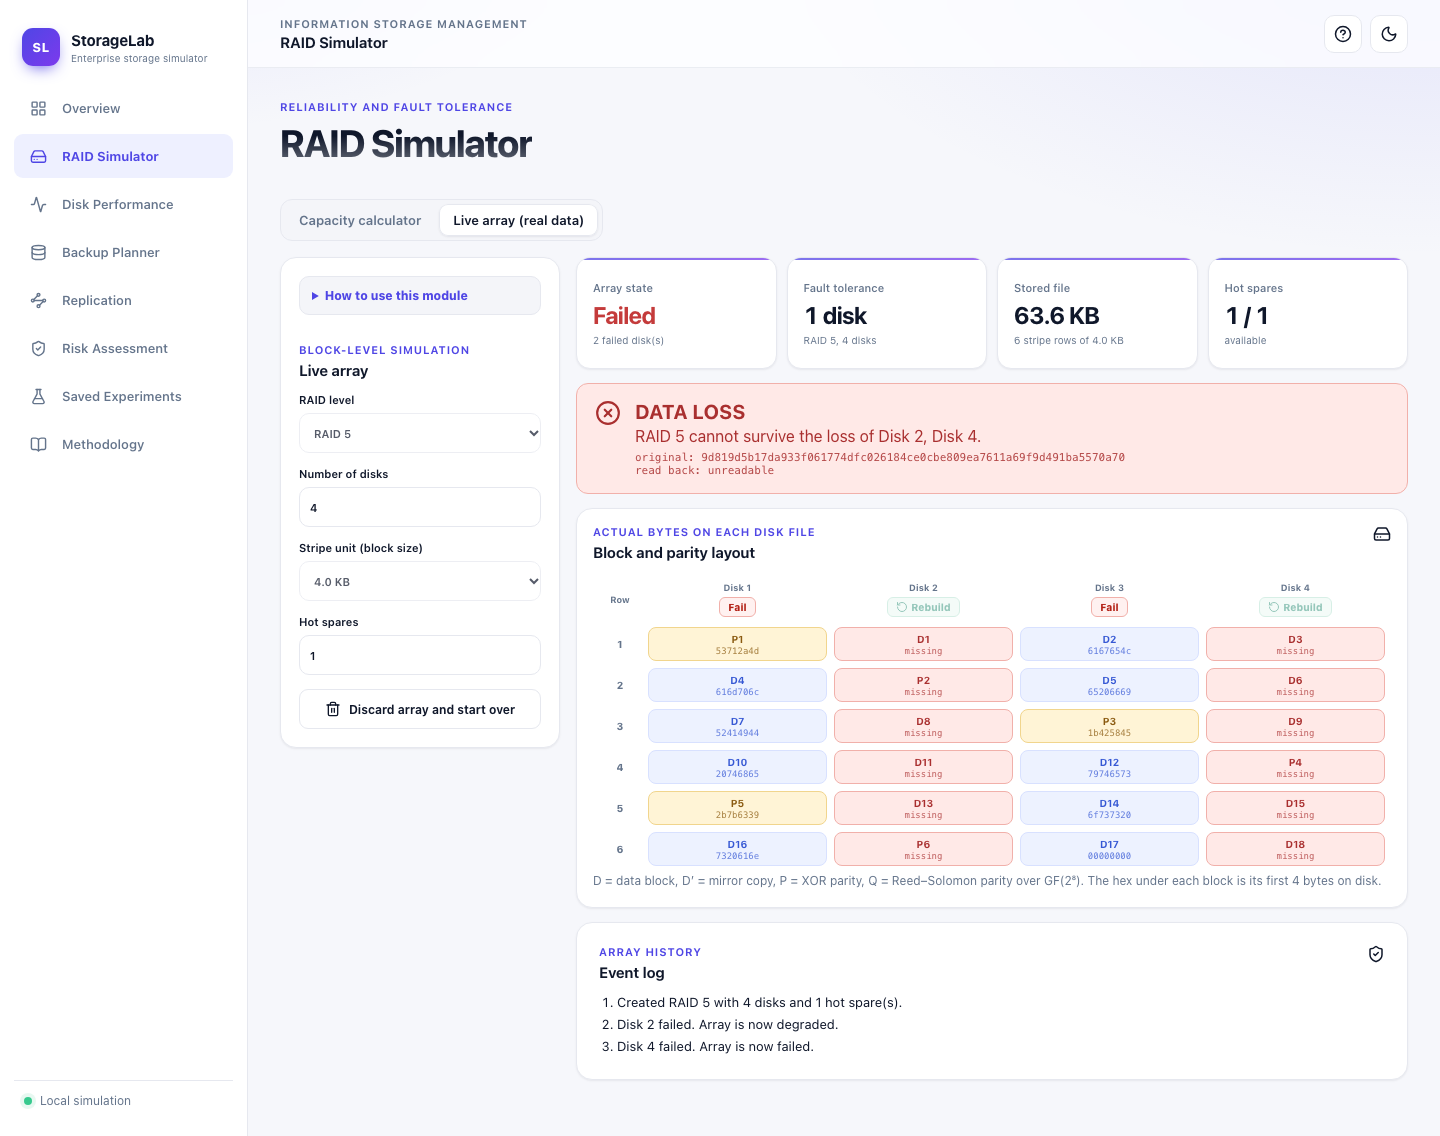
\includegraphics[width=\columnwidth]{fig_live_array.png}
\caption{Live array panel. Each cell shows the role of a stored block and its first bytes as read from the disk file.}
\label{fig:live}
\end{figure}

% V. ANALYTICAL MODELS AND EXPLANATION LAYER
\section{Analytical Models and Explanation Layer}
\label{sec:models}

% V-A. RAID Capacity Calculator
\subsection{RAID Capacity Calculator}
For $N$ disks of size $S$, the calculator reports the values in Table~\ref{tab:raidcap}, using the write penalties of \cite{emc2012ism}. It accepts 2 to 32 disks. Efficiency is usable capacity divided by raw capacity. The failure simulation reports one of four states: Healthy, Degraded, Rebuilding (only when the array is Degraded and a hot spare is enabled), and Failed, which is never rebuilt. With $f$ failed disks and a sequential rebuild throughput $T$ in MB/s (200 MB/s by default), the rebuild time in hours is \begin{equation} t_{\text{rebuild}} = \frac{S \cdot f \cdot 1024^2}{T \cdot 3600}, \label{eq:rebuild} \end{equation} with $S$ in TB. An XOR exercise lets the learner remove one of three binary blocks and recover it as the XOR of the parity and the survivors.

\begin{table}[!t]
\caption{RAID Capacity Model}
\label{tab:raidcap}
\centering
\footnotesize
\begin{tabular}{lllc}
\toprule
Level & Usable & Fault tolerance & Write penalty \\
\midrule
RAID 0 & $N S$ & 0 & 1 \\
RAID 1 & $N S/2$ & mirror-dependent & 2 \\
RAID 5 & $(N-1) S$ & 1 & 4 \\
RAID 6 & $(N-2) S$ & 2 & 6 \\
RAID 10 & $N S/2$ & mirror-dependent & 2 \\
\bottomrule
\end{tabular}
\end{table}

% V-B. Disk Performance
\subsection{Disk Performance}
A single disk is modeled as an M/M/1 queue \cite{kleinrock1975queueing}. With rotational speed RPM, average seek time $T_{\text{seek}}$, transfer rate $X$ in MB/s, and block size $B$ in KB, the times in milliseconds are \begin{align} T_{\text{rot}} &= \frac{30000}{\text{RPM}}, \qquad T_{\text{xfer}} = \frac{B/1024}{X} \cdot 1000, \\ T_s &= T_{\text{seek}} + T_{\text{rot}} + T_{\text{xfer}} , \end{align} where $T_{\text{rot}}$ is half a revolution. The maximum throughput is $1000/T_s$ IOPS. For an arrival rate $\lambda$ in IOPS, the utilization, response time, queue length, and number in the system are \begin{equation} U = \lambda T_s, \quad R = \frac{T_s}{1-U}, \quad L_q = \frac{U^2}{1-U}, \quad N = \lambda R = \frac{U}{1-U}, \label{eq:mm1} \end{equation} with $T_s$ in seconds for $U$; the last identity is Little's law \cite{little1961proof}. Inputs with $U \ge 1$ are rejected, and the error message gives the maximum stable arrival rate. The interface plots $R$ at 91 utilization points from 5\% to 95\%.

% V-C. Backup Planner
\subsection{Backup Planner}
The inputs are the data size $D$ in GB, the daily change rate $c$ in percent, the number of retained restore points $R$, the throughput in MB/s, the RPO, the RTO, and the backup interval. With daily change $C = D c/100$, the three strategies compare as shown in Table~\ref{tab:backupmodel}. Backup or restore duration in hours is the volume in GB times 1024, divided by the throughput and by 3600. The RPO is met if the interval does not exceed the RPO, and the RTO is met if the restore time does not exceed the RTO. Among the strategies that meet both, the planner recommends the one with the least retained storage. If none meets both, it says so explicitly and suggests increasing the backup frequency or throughput, or revising the objectives.

\begin{table}[!t]
\caption{Backup Strategy Model}
\label{tab:backupmodel}
\centering
\footnotesize
\setlength{\tabcolsep}{3pt}
\begin{tabular}{llll}
\toprule
 & Full & Incremental & Differential \\
\midrule
Retained & $R D$ & $D + (R-1) C$ & $D + \sum_{j=1}^{R-1} \min(jC, D)$ \\
Per backup & $D$ & $C$ & $\min((R-1)C, D)$ \\
Restore data & $D$ & $D + (R-1) C$ & $D + \min((R-1)C, D)$ \\
Restore steps & 1 & $R$ & 2 \\
\bottomrule
\end{tabular}
\end{table}

% V-D. Replication
\subsection{Replication}
For a distance $d$ in km, the propagation round-trip time is $2 \cdot d \cdot 0.005$ ms, using about 5~$\mu$s/km in fiber, and the total RTT adds the network RTT. A write of $W$ KB is $W \cdot 1024 \cdot 8$ bits, and its transmit time on a link of $L$ Mbps is the bit count divided by $L \cdot 10^6$, in milliseconds. The link utilization at a given write rate is \begin{equation} \rho = \frac{\text{IOPS} \cdot \text{bits}}{10^6 \cdot L}, \end{equation} and a saturated link ($\rho \ge 1$) is rejected. Synchronous replication has response time equal to the local write time plus the total RTT, with zero lag and an RPO of zero. Asynchronous replication responds after the local write, and its lag, which is also its RPO, is \begin{equation} \text{lag} = \frac{\text{RTT}_{\text{total}}}{2} + \frac{t_{\text{transmit}}}{1-\rho}, \label{eq:lag} \end{equation} where the second term is the M/M/1 sojourn time on the link. The number of writes at risk is the IOPS times the lag.

% V-E. Risk
\subsection{Risk}
The risk score is likelihood times impact, each an integer from 1 to 5. The bands are Low (1 to 5), Medium (6 to 10), High (11 to 15), and Critical (16 to 25). Mitigations are mapped per threat (hardware failure, ransomware, unauthorized access), with a generic fallback.

% V-F. Unit Conventions
\subsection{Unit Conventions}
Storage sizes are binary: 1 TB is $1024^2$ MB in the rebuild model and 1 GB is 1024 MB in the backup model. Network rates are decimal: 1 Mbps is $10^6$ bit/s, while a write size uses 1 KB = 1024 B. All times are converted to consistent units before division: milliseconds within a disk operation and hours for backup and rebuild.

% V-G. Explanation Layer
\subsection{Explanation Layer}
Each module returns an explanation object with a summary, the formula, the contributing factors, and the assumptions. The text is built from the same computed values that the response returns, so it is always consistent with the numbers. The layer is a deterministic, rule-based template system, not a learned model, which makes every explanation reproducible and checkable against the formulas in this section.

% VI. VALIDATION AND RESULTS
\section{Validation and Results}
\label{sec:eval}

All measurements were taken on an Apple M5 laptop with 16 GB of RAM, running macOS, Python 3.15.2, and NumPy 2.5.5. Each timing is the median of five runs. Every number in this section is reproduced by a single measurement script in the project repository.

% VI-A. Automated Tests
\subsection{Automated Tests}
The Python suite contains 62 tests, which pass in 0.80 s, and the front end has 11 Vitest tests, which also pass. Module tests check the RAID capacity of every level, invalid configurations, failure states, write penalties, XOR recovery, rebuild time, the disk formulas against hand-calculated values, queue length, rejection of unstable utilization, backup storage and RPO/RTO compliance, replication distance and lag units, link saturation, and risk bands. The RAID engine tests check that a write followed by a read returns identical bytes for every level; that every combination of failures up to the level's tolerance, including every pair for RAID 6, is read in degraded mode and rebuilt onto spares with a matching SHA-256 digest and a Healthy state; that failures beyond tolerance report data loss and refuse rebuild; that each RAID 5 parity block equals the XOR of its row and that parity rotates; and the GF inverse and scaling identities. API tests exercise the end-to-end flow of create, fail, verify, rebuild, and verify.

% VI-B. Exhaustive Fault-Injection Campaign
\subsection{Exhaustive Fault-Injection Campaign}
For each of 14 configurations, every non-empty subset of disks ($2^n - 1$ subsets) was failed on a fresh array holding a 16 KiB random file with a 512 B stripe unit. After a read, the SHA-256 digest was compared with the original, and each outcome was classified as recovered, reported data loss, or silent mismatch, meaning the read succeeded but the bytes differ. The observed outcome was also compared with the predicate (\ref{eq:pred}).

Table~\ref{tab:campaign} shows the results. Of 1,058 failure combinations, 219 were recovered byte-exactly, 839 were correctly reported as data loss, and none produced a silent mismatch. The predicate agreed with the observed outcome in all 1,058 cases.

The recovered counts also match the combinatorics, which serves as a sanity check. RAID 5 recovers exactly the $n$ single failures. RAID 6 recovers the $\binom{n}{1} + \binom{n}{2}$ subsets of size one or two, for example $8 + 28 = 36$ at $n=8$. RAID 10 recovers $3^{n/2} - 1$ subsets, because each mirror pair can lose nothing, its first member, or its second member, which gives 80 at $n = 8$. This answers RQ1: within its tolerance the engine recovers byte-exactly, and beyond it the engine reports data loss rather than returning wrong data.

\begin{table}[!t]
\caption{Exhaustive Fault-Injection Results}
\label{tab:campaign}
\centering
\footnotesize
\setlength{\tabcolsep}{4pt}
\begin{tabular}{lrrrrr}
\toprule
Config. & Subsets & Recovered & Data loss & Silent & Agreement \\
\midrule
RAID 0, $n$=2 & 3 & 0 & 3 & 0 & 3/3 \\
RAID 0, $n$=4 & 15 & 0 & 15 & 0 & 15/15 \\
RAID 1, $n$=2 & 3 & 2 & 1 & 0 & 3/3 \\
RAID 5, $n$=3 & 7 & 3 & 4 & 0 & 7/7 \\
RAID 5, $n$=4 & 15 & 4 & 11 & 0 & 15/15 \\
RAID 5, $n$=6 & 63 & 6 & 57 & 0 & 63/63 \\
RAID 5, $n$=8 & 255 & 8 & 247 & 0 & 255/255 \\
RAID 6, $n$=4 & 15 & 10 & 5 & 0 & 15/15 \\
RAID 6, $n$=5 & 31 & 15 & 16 & 0 & 31/31 \\
RAID 6, $n$=6 & 63 & 21 & 42 & 0 & 63/63 \\
RAID 6, $n$=8 & 255 & 36 & 219 & 0 & 255/255 \\
RAID 10, $n$=4 & 15 & 8 & 7 & 0 & 15/15 \\
RAID 10, $n$=6 & 63 & 26 & 37 & 0 & 63/63 \\
RAID 10, $n$=8 & 255 & 80 & 175 & 0 & 255/255 \\
\midrule
Total & 1,058 & 219 & 839 & 0 & 1,058/1,058 \\
\bottomrule
\end{tabular}
\end{table}

% VI-C. Model Case Studies
\subsection{Model Case Studies}
% --- VI-C-1. RAID Capacity ---
\subsubsection{RAID Capacity}
For eight 4 TB disks, the calculator reports usable capacities of 32, 16, 28, 24, and 16 TB for RAID 0, 1, 5, 6, and 10, corresponding to efficiencies of 100\%, 50\%, 87.5\%, 75\%, and 50\% and write penalties of 1, 2, 4, 6, and 2.

% --- VI-C-2. Disk Performance ---
\subsubsection{Disk Performance}
For a 7200 RPM disk with a 4 ms seek, a 150 MB/s transfer rate, and 4 KB blocks, the service time is 8.193 ms and the maximum throughput is 122.06 IOPS. Table~\ref{tab:disk} shows the metrics as the arrival rate rises. The step from 61\% to 82\% utilization doubles the response time from 21.3 ms to 45.3 ms, which illustrates the knee of the curve, and an arrival rate of 125 IOPS is rejected because it would give $U = 102.4\%$.

\begin{table}[!t]
\caption{Disk Metrics at 7200 RPM ($T_s$ = 8.193 ms)}
\label{tab:disk}
\centering
\footnotesize
\begin{tabular}{rrrrr}
\toprule
$\lambda$ (IOPS) & $U$ (\%) & $R$ (ms) & $L_q$ & $N$ \\
\midrule
0 & 0.00 & 8.193 & 0.000 & 0.000 \\
25 & 20.48 & 10.303 & 0.053 & 0.258 \\
50 & 40.96 & 13.877 & 0.284 & 0.694 \\
75 & 61.45 & 21.250 & 0.979 & 1.594 \\
100 & 81.93 & 45.331 & 3.714 & 4.533 \\
125 & \multicolumn{4}{l}{rejected ($U = 102.4\%$)} \\
\bottomrule
\end{tabular}
\end{table}

Spindle speed has a strong effect near saturation (Fig.~\ref{fig:rpm} and Table~\ref{tab:rpm}). At 100 IOPS, the 1.4 ms difference in service time between 7200 and 5400 RPM produces a five-fold difference in response time, from 45.3 ms to 229.0 ms.

\begin{table}[!t]
\caption{Effect of Spindle Speed at $\lambda$ = 100 IOPS}
\label{tab:rpm}
\centering
\footnotesize
\begin{tabular}{rrrrr}
\toprule
RPM & $T_{\text{rot}}$ (ms) & $T_s$ (ms) & $U$ (\%) & $R$ (ms) \\
\midrule
5400 & 5.556 & 9.582 & 95.8 & 229.004 \\
7200 & 4.167 & 8.193 & 81.9 & 45.331 \\
10000 & 3.000 & 7.026 & 70.3 & 23.625 \\
15000 & 2.000 & 6.026 & 60.3 & 15.164 \\
\bottomrule
\end{tabular}
\end{table}

\begin{figure}[!t]
\centering
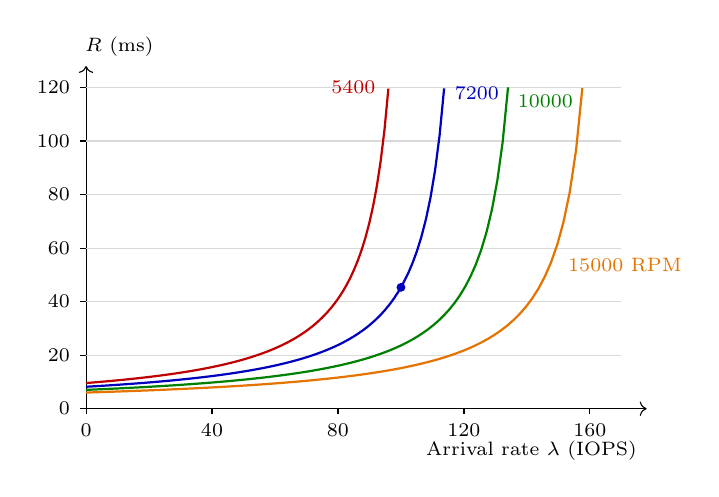
\begin{tikzpicture}[x=0.040cm, y=0.034cm, font=\scriptsize]
\draw[->] (0,0) -- (178,0) node[below left, yshift=-8pt] {Arrival rate $\lambda$ (IOPS)};
\draw[->] (0,0) -- (0,128) node[above, xshift=12pt] {$R$ (ms)};
\foreach \x in {0,40,80,120,160} \draw (\x,0) -- (\x,-2) node[below] {\x};
\foreach \y in {0,20,40,60,80,100,120} \draw (0,\y) -- (-2,\y) node[left] {\y};
\draw[gray!30] (0,20) -- (170,20) (0,40) -- (170,40) (0,60) -- (170,60) (0,80) -- (170,80) (0,100) -- (170,100) (0,120) -- (170,120);
\draw[thick, red!75!black, domain=0:96.0, samples=80] plot (\x, {9.582/(1-\x*9.582/1000)});
\draw[thick, blue!75!black, domain=0:113.7, samples=80] plot (\x, {8.193/(1-\x*8.193/1000)});
\draw[thick, green!50!black, domain=0:134.0, samples=80] plot (\x, {7.026/(1-\x*7.026/1000)});
\draw[thick, orange!90!black, domain=0:157.6, samples=80] plot (\x, {6.026/(1-\x*6.026/1000)});
\node[red!75!black, anchor=east] at (95,120) {5400};
\node[blue!75!black, anchor=west] at (114,118) {7200};
\node[green!50!black, anchor=west] at (134,115) {10000};
\node[orange!90!black, anchor=north west] at (150,60) {15000 RPM};
\fill[blue!75!black] (100,45.331) circle (1.6pt);
\end{tikzpicture}
\caption{Response time against arrival rate for four spindle speeds (4 ms seek, 150 MB/s, 4 KB blocks). The dot marks 100 IOPS at 7200 RPM.}
\label{fig:rpm}
\end{figure}

% --- VI-C-3. Backup ---
\subsubsection{Backup}
For 1000 GB of data with 5\% daily change, seven retained points, a throughput of 100 MB/s, daily backups, an RPO of 24 h, and an RTO of 4 h, the planner produces Table~\ref{tab:backup}. All three strategies meet both objectives, and the planner recommends incremental backup because it needs the least retained storage. With an RPO of 1 h and daily backups, no strategy is compliant, and the system says so explicitly.

\begin{table*}[!t]
\caption{Backup Case Study (1000 GB, 5\%/day, 7 Points, 100 MB/s, RPO 24 h, RTO 4 h)}
\label{tab:backup}
\centering
\footnotesize
\begin{tabular}{lrrrrrcc}
\toprule
Strategy & Retained (GB) & Backup (h) & Restore (h) & Restore data (GB) & Steps & RPO met & RTO met \\
\midrule
Full & 7000 & 2.844 & 2.844 & 1000 & 1 & Yes & Yes \\
Incremental & 1300 & 0.142 & 3.698 & 1300 & 7 & Yes & Yes \\
Differential & 2050 & 0.853 & 3.698 & 1300 & 2 & Yes & Yes \\
\bottomrule
\end{tabular}
\end{table*}

% --- VI-C-4. Replication ---
\subsubsection{Replication}
With a 2 ms local write, a 2 ms network RTT, a 1000 Mbps link, 500 IOPS, and 8 KB writes ($\rho = 3.28\%$), synchronous response time grows linearly with distance while asynchronous response stays at the local write time (Table~\ref{tab:repl} and Fig.~\ref{fig:repl}). The asynchronous lag, and therefore the RPO, also grows with distance. At 100 km, reducing the bandwidth raises the lag from 1.568 ms at 1000 Mbps ($\rho = 3.3\%$) to 2.475 ms at 100 Mbps ($\rho = 32.8\%$), 5.303 ms at 50 Mbps ($\rho = 65.5\%$), and 10.562 ms at 40 Mbps ($\rho = 81.9\%$). Below about 32.8 Mbps the link saturates and the input is rejected.

\begin{table}[!t]
\caption{Replication Against Distance}
\label{tab:repl}
\centering
\footnotesize
\begin{tabular}{rrrr}
\toprule
Distance & Sync. response & Async. response & Async. lag/RPO \\
(km) & (ms) & (ms) & (ms) \\
\midrule
0 & 4.000 & 2.000 & 1.068 \\
10 & 4.100 & 2.000 & 1.118 \\
100 & 5.000 & 2.000 & 1.568 \\
500 & 9.000 & 2.000 & 3.568 \\
1000 & 14.000 & 2.000 & 6.068 \\
5000 & 54.000 & 2.000 & 26.068 \\
\bottomrule
\end{tabular}
\end{table}

\begin{figure}[!t]
\centering
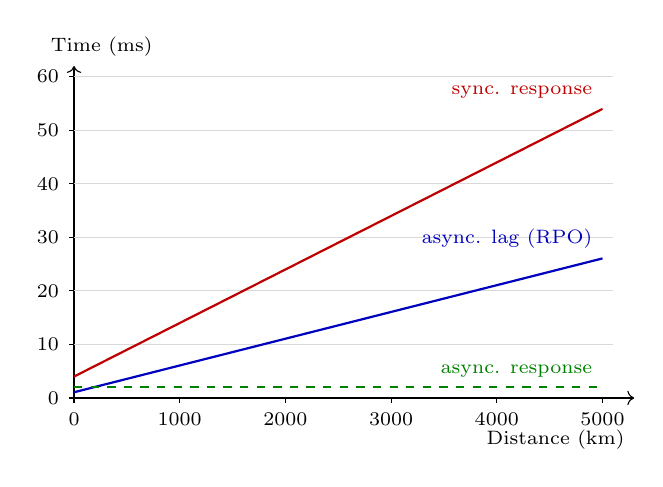
\begin{tikzpicture}[x=0.00135cm, y=0.068cm, font=\scriptsize]
\draw[->] (0,0) -- (5300,0) node[below left, yshift=-8pt] {Distance (km)};
\draw[->] (0,0) -- (0,62) node[above, xshift=10pt] {Time (ms)};
\foreach \x in {0,1000,2000,3000,4000,5000} \draw (\x,0) -- (\x,-1) node[below] {\x};
\foreach \y in {0,10,20,30,40,50,60} \draw (0,\y) -- (-50,\y) node[left] {\y};
\draw[gray!30] (0,10) -- (5100,10) (0,20) -- (5100,20) (0,30) -- (5100,30) (0,40) -- (5100,40) (0,50) -- (5100,50) (0,60) -- (5100,60);
\draw[thick, red!75!black] (0,4) -- (5000,54) node[above left] {sync. response};
\draw[thick, blue!75!black] (0,1.068) -- (5000,26.068) node[above left] {async. lag (RPO)};
\draw[thick, green!50!black, dashed] (0,2) -- (5000,2) node[above left] {async. response};
\end{tikzpicture}
\caption{Synchronous response time, asynchronous response time, and asynchronous lag against distance (1000 Mbps, 500 IOPS, 8 KB writes).}
\label{fig:repl}
\end{figure}

% VI-D. Engine Performance
\subsection{Engine Performance}
Table~\ref{tab:perf} reports engine timings for a 4 MiB random file, excluding the interface's artificial rebuild delay. Every operation finishes within 25 ms, well below interactive thresholds, on a laptop with no special privileges, which answers RQ3. RAID 6 encoding and recovery take about four to five times longer than RAID 5 because of the GF($2^8$) multiplications, which are table lookups, compared with a single XOR for P. This mirrors the real computational overhead of RAID 6 and its higher write penalty. The measured ratio of raw to file bytes is slightly above the theoretical $n/k$ (1.333 for RAID 5 with four disks and 1.667 for RAID 6 with five disks) because of zero padding in the last row. The padding grows with the stripe unit, which gives a concrete way to discuss internal fragmentation. These timings are in-memory NumPy timings on page-cached files, not device benchmarks.

\begin{table*}[!t]
\caption{Engine Timings for a 4 MiB File (Seconds, Median of 5 Runs)}
\label{tab:perf}
\centering
\footnotesize
\begin{tabular}{llrrrrrrr}
\toprule
Level, $n$ & Unit & Rows & Encode & Read & Degraded read & Rebuild 1 disk & Read, 2 failed & Raw/file bytes \\
\midrule
RAID 0, 4 & 4 KiB & 256 & 0.003 & 0.001 & -- & -- & -- & 1.000 \\
RAID 0, 4 & 64 KiB & 16 & 0.002 & 0.001 & -- & -- & -- & 1.000 \\
RAID 1, 2 & 4 KiB & 1024 & 0.005 & 0.002 & 0.003 & 0.002 & -- & 2.000 \\
RAID 1, 2 & 64 KiB & 64 & 0.004 & 0.001 & 0.001 & 0.001 & -- & 2.000 \\
RAID 5, 4 & 4 KiB & 342 & 0.004 & 0.001 & 0.004 & 0.003 & -- & 1.336 \\
RAID 5, 4 & 64 KiB & 22 & 0.004 & 0.001 & 0.002 & 0.002 & -- & 1.375 \\
RAID 6, 5 & 4 KiB & 342 & 0.019 & 0.001 & 0.017 & 0.017 & 0.025 & 1.670 \\
RAID 6, 5 & 64 KiB & 22 & 0.015 & 0.001 & 0.013 & 0.013 & 0.019 & 1.719 \\
RAID 10, 4 & 4 KiB & 512 & 0.004 & 0.001 & 0.002 & 0.002 & -- & 2.000 \\
RAID 10, 4 & 64 KiB & 32 & 0.003 & 0.001 & 0.001 & 0.001 & -- & 2.000 \\
\bottomrule
\end{tabular}
\end{table*}

% VI-E. Demonstration Scenario
\subsection{Demonstration Scenario}
A typical classroom session runs as follows. The instructor creates a RAID 5 array with four disks, a 4 KiB stripe unit, and one spare, and shows P rotating across the disks row by row. Failing Disk 2 moves the array to the Degraded state, yet the SHA-256 digest still matches because the missing blocks are reconstructed on every read. Rebuilding Disk 2 streams a progress bar, the spare becomes Disk 2, the state returns to Healthy, and the digest matches again. Failing two disks of a RAID 5 array produces a data-loss report and a refused rebuild, whereas the same two failures on a five-disk RAID 6 array still give a matching digest. The session continues with the capacity comparison and the XOR exercise, raises the disk arrival rate past the 70\% knee, and shows a backup plan with an RPO of 1 h failing under daily backups and passing under hourly backups.

% VII. DISCUSSION AND LIMITATIONS
\section{Discussion and Limitations}
\label{sec:disc}

The results answer the three research questions within clear limits, which are stated here.

% VII-A. RAID Engine
\subsection{RAID Engine}
The engine corrects erasures, meaning disks known to be missing, not silent errors. It keeps no per-block checksums, so it cannot detect or locate bit rot inside a surviving disk; the SHA-256 digest only detects end-to-end corruption. The engine is file-backed rather than block-device-backed and models no controller cache, write hole, partial-stripe read-modify-write, or concurrent I/O. Whole disks are loaded into memory, so scalability relies on the 5 MiB and eight-disk limits. The parity layout is a simple rotation rather than the left-symmetric layout of Linux md or a vendor layout. The metadata file has no locking, so concurrent changes to the same array could race; this is acceptable for a single-user teaching tool. Finally, the API slows rebuilds artificially so that progress is visible.

% VII-B. Analytical Models
\subsection{Analytical Models}
The disk model is M/M/1 with exponential service. Real disk service is closer to a general distribution, so an M/G/1 model or measured traces would be more faithful, and the model covers a single disk with no scheduler, cache, or array-level aggregation. The write penalty is reported but not yet combined with disk IOPS. In the backup model with a fixed daily change, incremental and differential backups restore the same data volume and differ only in restore steps and retained storage; RPO compliance depends only on the interval, not on the backup duration; and deduplication and compression are not modeled. The replication model assumes one transfer per write, a constant propagation speed, and no protocol overhead, and models the link as an M/M/1 queue. Risk scores come from judgment rather than measured frequencies, and the rebuild time assumes a constant sequential throughput.

% VII-C. Evaluation
\subsection{Evaluation}
No user study has been conducted yet, so this paper makes claims only about correctness and performance, not about learning outcomes. \todo{Add the results of a pre-test and post-test study with control and treatment groups, and a System Usability Scale questionnaire, if run before submission.}

% VII-D. Security
\subsection{Security}
The system has no authentication, restricts cross-origin requests to local origins, limits uploads to 5 MiB, and validates array identifiers to prevent path traversal. It is intended for local or classroom deployment.

% VIII. CONCLUSION AND FUTURE WORK
\section{Conclusion and Future Work}
\label{sec:concl}
StorageLab shows that a lightweight, pure-software laboratory can make storage concepts both computable and observable. Its file-backed RAID engine stripes real data with RAID 0, 1, 5, 6, and 10, reconstructs every single and double erasure in closed form, and proves each recovery with a SHA-256 match. An exhaustive campaign over 1,058 failure combinations found no silent corruption and complete agreement with the recoverability predicate. The analytical models return values with units, assumptions, and formula-grounded explanations, and every engine operation on a 4 MiB file completes within 25 ms on a laptop.

Future work includes, first and most important, a pedagogical evaluation with pre-tests and post-tests, control and treatment groups, and a usability questionnaire. Further extensions are per-block checksums and scrubbing, so that the engine can demonstrate silent-corruption detection and correction with RAID 6; array-level IOPS that combine the write penalty with disk performance, through the effective front-end rate $n \cdot \text{IOPS}_{\text{disk}} / (r + w \cdot \text{penalty})$ for read and write fractions $r$ and $w$; an M/G/1 disk model and workload traces; general Reed-Solomon $(k+m)$ codes, locally repairable codes, and declustered parity rebuild; a rebuild-window risk model based on the mean time to failure and the mean time to repair; and a multi-user deployment with authentication and per-user workspaces.

% ACKNOWLEDGMENT
\section*{Acknowledgment}
\todo{Acknowledgments, if any.}

% REFERENCES
\begin{thebibliography}{00}

\bibitem{patterson1988raid} D. A. Patterson, G. Gibson, and R. H. Katz, ``A case for redundant arrays of inexpensive disks (RAID),'' in \emph{Proc. ACM SIGMOD Int. Conf. Manage. Data}, Chicago, IL, USA, 1988, pp. 109--116.

\bibitem{chen1994raid} P. M. Chen, E. K. Lee, G. A. Gibson, R. H. Katz, and D. A. Patterson, ``RAID: High-performance, reliable secondary storage,'' \emph{ACM Comput. Surv.}, vol. 26, no. 2, pp. 145--185, Jun. 1994.

\bibitem{reed1960polynomial} I. S. Reed and G. Solomon, ``Polynomial codes over certain finite fields,'' \emph{J. Soc. Ind. Appl. Math.}, vol. 8, no. 2, pp. 300--304, 1960.

\bibitem{plank1997tutorial} J. S. Plank, ``A tutorial on Reed-Solomon coding for fault-tolerance in RAID-like systems,'' \emph{Softw. Pract. Exper.}, vol. 27, no. 9, pp. 995--1012, 1997.

\bibitem{anvin2004raid6} H. P. Anvin, ``The mathematics of RAID-6,'' 2004. [Online]. Available: https://www.kernel.org/pub/linux/kernel/people/hpa/raid6.pdf

\bibitem{little1961proof} J. D. C. Little, ``A proof for the queuing formula: $L = \lambda W$,'' \emph{Oper. Res.}, vol. 9, no. 3, pp. 383--387, 1961.

\bibitem{kleinrock1975queueing} L. Kleinrock, \emph{Queueing Systems, Volume 1: Theory}. New York, NY, USA: Wiley, 1975.

\bibitem{ruemmler1994disk} C. Ruemmler and J. Wilkes, ``An introduction to disk drive modeling,'' \emph{Computer}, vol. 27, no. 3, pp. 17--28, Mar. 1994.

\bibitem{bucy2008disksim} J. S. Bucy, J. Schindler, S. W. Schlosser, and G. R. Ganger, ``The DiskSim simulation environment version 4.0 reference manual,'' Parallel Data Lab., Carnegie Mellon Univ., Pittsburgh, PA, USA, Tech. Rep. CMU-PDL-08-101, May 2008.

\bibitem{emc2012ism} EMC Education Services, \emph{Information Storage and Management: Storing, Managing, and Protecting Digital Information in Classic, Virtualized, and Cloud Environments}, 2nd ed. Indianapolis, IN, USA: Wiley, 2012.

\end{thebibliography}

% AUTHOR BIOGRAPHIES
\begin{IEEEbiography}[{
\includegraphics[width=1in,height=1.25in,clip,keepaspectratio]{a1.png}}]{First Author}
\todo{Author biography and photograph.}
\end{IEEEbiography}

\begin{IEEEbiography}[{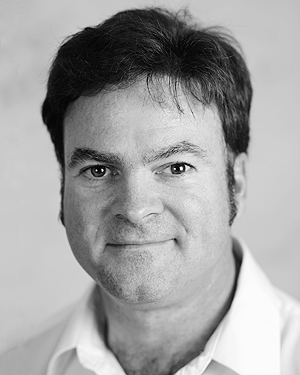
\includegraphics[width=1in,height=1.25in,clip,keepaspectratio]{a2.png}}]{Second Author}
\todo{Author biography and photograph.}
\end{IEEEbiography}

\begin{IEEEbiography}[{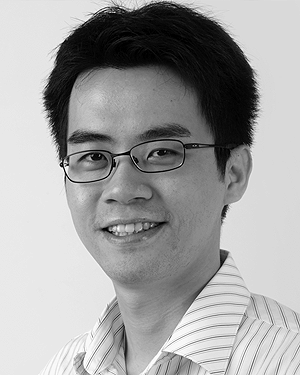
\includegraphics[width=1in,height=1.25in,clip,keepaspectratio]{a3.png}}]{Third Author}
\todo{Author biography and photograph.}
\end{IEEEbiography}

\EOD

\end{document}
